\subsection{Overview}

\begin{figure*}[ht]
  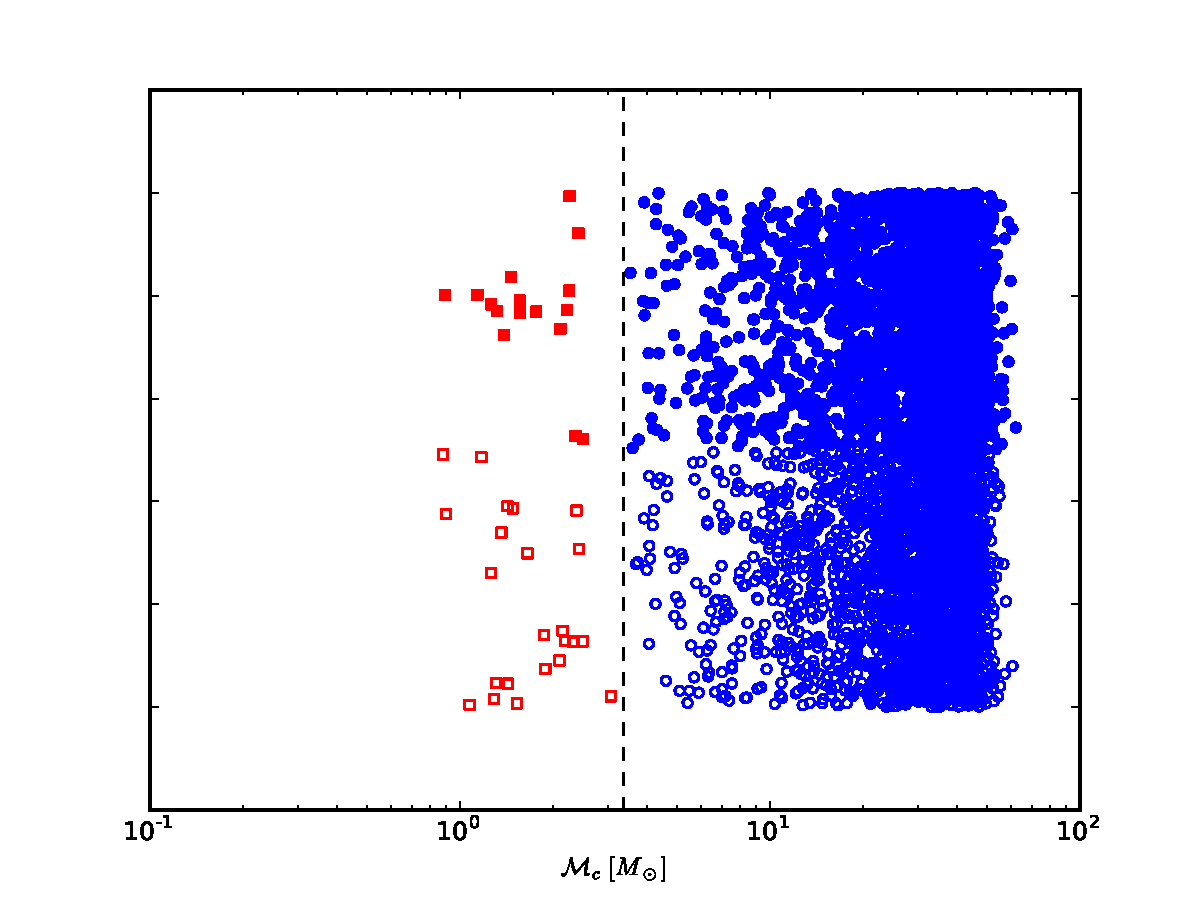
\includegraphics[width=\textwidth]{img/classifier_comparison}
  \caption{Visualization of 1D classifier performance. Red points have observed EM counterparts, while blue do not. We trained the classifier only on the data with solid points, and obtained a decision boundary shown by the dashed line. The open points are the remaining half of the data, which, as you can see, were correctly classified by this decision boundary.}
  \label{fig:class}
\end{figure*}

\begin{figure*}[ht]
  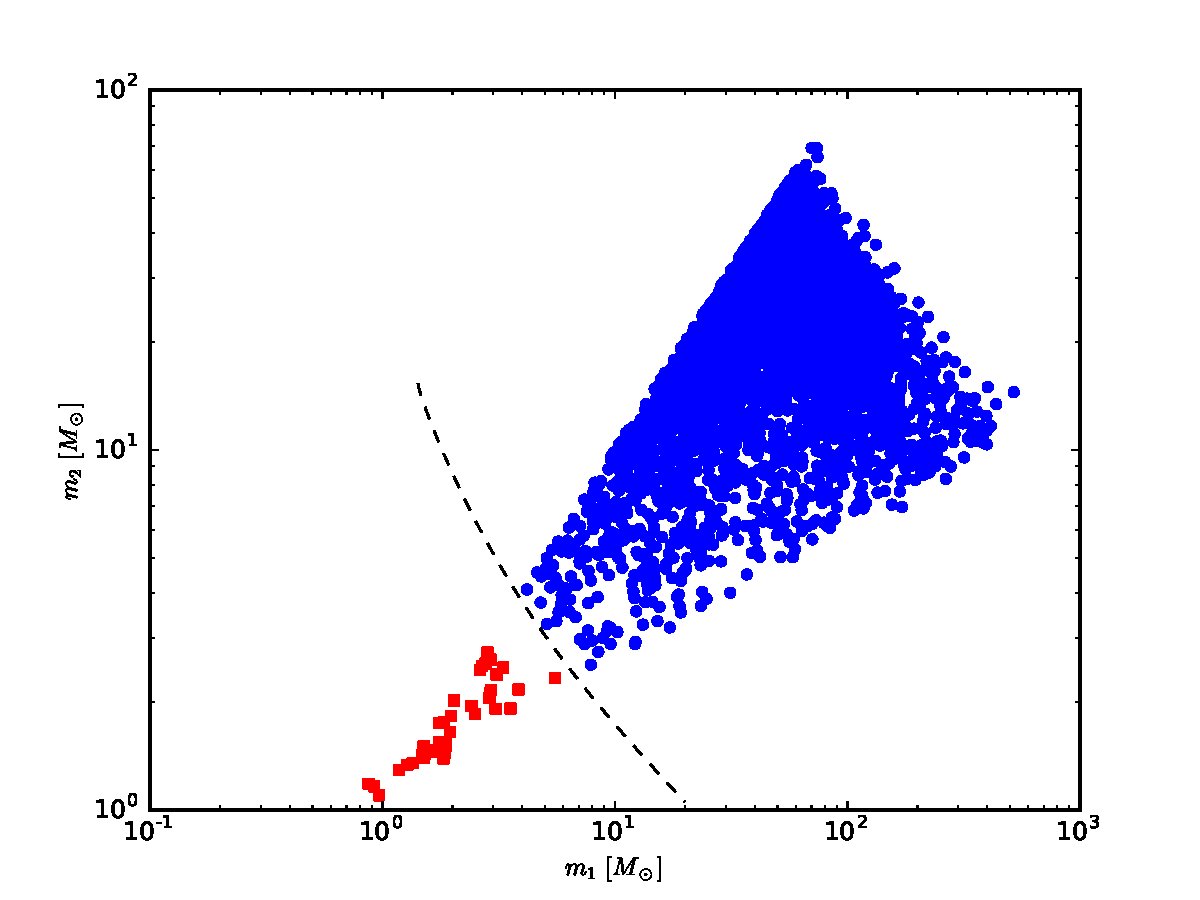
\includegraphics[width=\textwidth]{img/mass-distribution}
  \caption{Decision boundary from 1D classifier trained on $\mathcal{M}_c$, overlayed on the 2D mass distribution. Red points have EM counterparts, while blue do not.}
  \label{fig:2D}
\end{figure*}

\begin{figure*}[ht]
  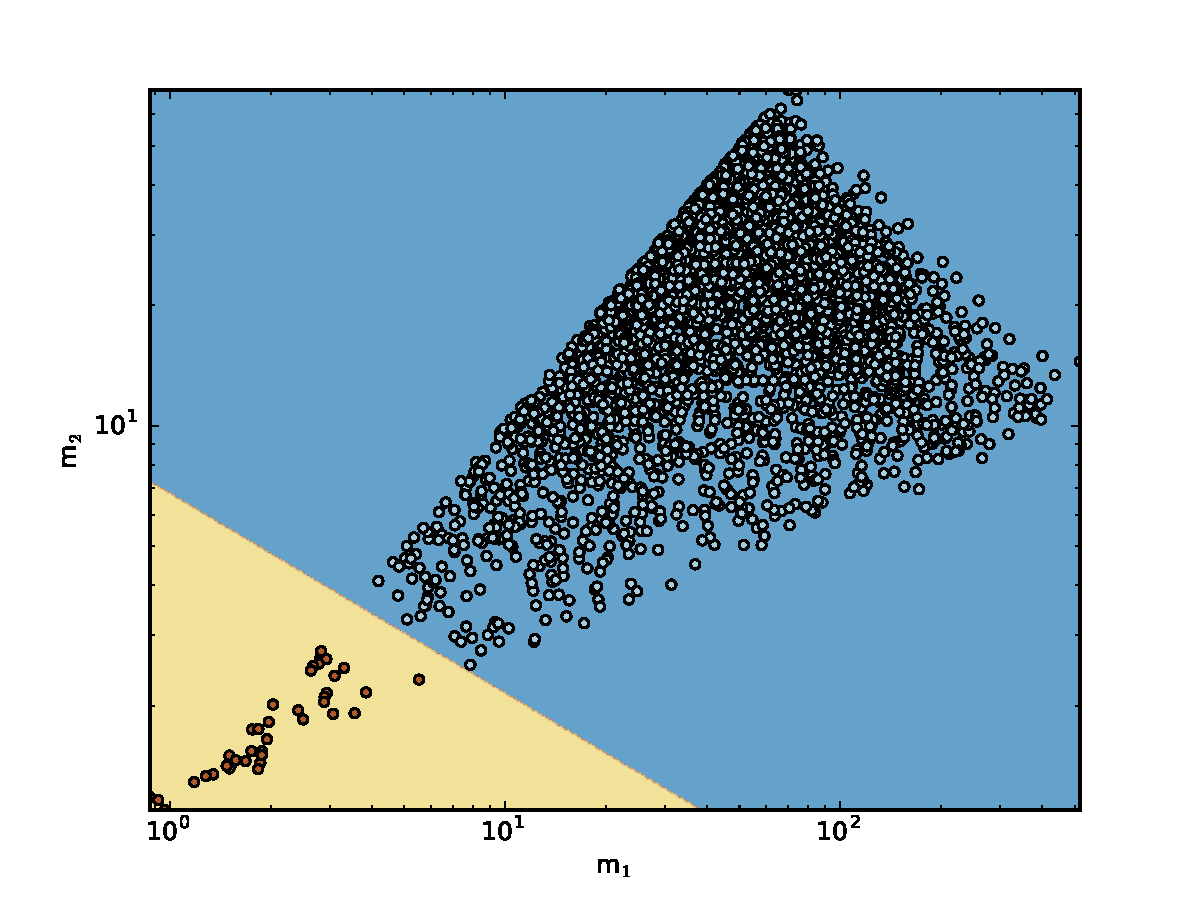
\includegraphics[width=\textwidth]{img/classifier-2D.pdf}
  \caption{Results of linear SVM classifier, trained on half of the data set, displayed here to perfectly classify the entire data set. Red points represent events with EM counterparts, and blue points represent the events without. The predictions of the classifier are shown as the yellow and blue shaded regions.}
  \label{fig:2dclass}
\end{figure*}



LIGO can provide very rapid mass estimates of candidate GW events. Since most of these detections are binary black holes, and EM followup is extremely expensive, very few events are expected to have confirmed EM counterparts.

We have trained a classifier to determine if an event will have a EM counterpart. In \S\ref{sec:classifier-method} we discuss the method used, and in \S\ref{sec:classifier-results} we discuss our results.


\subsection{Method}
\label{sec:classifier-method}
We trained this classifier on the first half of the data, simply taking the mid-way point in $\mathcal{M}_c$ between the population of events with EM counterparts and without. This is demonstrated in Figure \ref{fig:class}.

We took a slightly different approach for the 2D mass distribution, as part of the \textbf{500\% extra credit} problem. Here we trained a linear SVM, using \texttt{sklearn.svm.LinearSVC}, with \texttt{C=100}, and the masses transformed into log-space. Again, we performed the training on half of the data, and made correct predictions on the full data set. The results are shown in Figure \ref{fig:2dclass}.


\subsection{Results}
\label{sec:classifier-results}

The classifier correctly separated the two groups with $100\%$ completeness and zero contamination, even when the training was done using only half of the data set. Of course, this is potentially sensitive to precisely \emph{which} half of the data set was used, so one can imagine a likely scenario where this failed.

Looking at Figure \ref{fig:chirp}, you can see that the decision boundary occurs in one of the histogram bins with zero observations. In this sense, it does correlate with structure in the data.

In Figure \ref{fig:2D}, we have plotted that same decision boundary over the 2D mass distribution. To do this, we had to derive an expression for $m_2(m_1, \mathcal{M}_c)$, which we accomplished using \texttt{Mathematica}. The expression is
%
\begin{equation}
  m_2(m_1, \mathcal{M}_c) =
  \frac{(2/3)^{1/3} \mathcal{M}_c^5}{X} +
  \frac{X}{2^{1/3} \cdot 3^{2/3} \cdot m_1^3},
%
  \label{eq:m2-m1-Mc}
\end{equation}
%
where
%
\begin{equation}
  X \equiv
  \qty[
    9 m_1^7 \mathcal{M}_c^5 +
    \sqrt{3 m_1^9 \mathcal{M}_c^{10} \qty(27 m_1^5 - 4 \mathcal{M}_c^3)}
  ]^{1/3}.
\end{equation}
%
As you can see from Figure \ref{fig:2D}, this line corresponds to the division between the events with and without counterparts.

A similar result is obtained using the linear SVM on the 2D mass distribution directly. The result is shown in Figure \ref{fig:2dclass}.